\section{Module 4: Lưu trữ Bền vững \& Phục hồi Thảm họa với Snapshot}

\subsection{Mục tiêu \& Mô hình Lưu trữ Lai (Hybrid Storage)}
Trong kiến trúc điện toán đám mây hiện đại, nguyên lý cốt lõi là tách biệt hoàn toàn giữa các nút tính toán tạm thời (Ephemeral Compute Nodes) và lớp lưu trữ trạng thái bền vững (Persistent Storage State). Để hiện thực hóa mô hình này, nhóm chúng em triển khai kiến trúc lưu trữ lai (Hybrid Storage Model) kết hợp linh hoạt giữa hai dịch vụ nền tảng của OpenStack:
\begin{itemize}
    \item \textbf{Lưu trữ Đối tượng (OpenStack Swift)~\cite{swift_storage}:} Đóng vai trò kho lưu trữ tài nguyên phi cấu trúc và các gói phân phối mã nguồn tĩnh thông qua giao thức RESTful API, cho phép các tiến trình máy ảo truy xuất nhanh qua HTTP.
    \item \textbf{Lưu trữ Khối (OpenStack Cinder)~\cite{cinder_storage}:} Cung cấp các thiết bị khối chuẩn POSIX với độ trễ thấp và băng thông cao, được gắn trực tiếp vào máy ảo làm không gian thực thi dữ liệu ứng dụng.
    \item \textbf{Cơ chế Phục hồi Thảm họa (Snapshot Lifecycle):} Thực hiện chụp ảnh trạng thái ổ đĩa theo thời điểm (Point-in-time Snapshot), làm tiền đề cho việc nhân bản môi trường hoặc khôi phục dữ liệu tức thời khi máy ảo tính toán gặp sự cố phần cứng.
\end{itemize}

\subsection{Thiết lập Swift Object Storage}
Bước đầu tiên trong quy trình, nhóm chúng em tiến hành thiết lập OpenStack Swift để làm kênh phân phối mã nguồn cho ứng dụng:
\begin{itemize}
    \item \textbf{Khởi tạo Container:} Chúng em tạo một container chuyên dụng mang tên \nolinkurl{module4-tetris-src} áp dụng chính sách lưu trữ mặc định \texttt{Policy-0}, đồng thời thiết lập quyền truy cập đọc công khai (\nolinkurl{Read-ACL=.r:*}) nhằm cho phép các node trong mạng nội bộ tải tài nguyên mà không cần truyền token xác thực phức tạp.
    \item \textbf{Tải lên Đối tượng:} Tệp mã nguồn giao diện \texttt{index.html} (kích thước 247 bytes) được nhóm chúng em tải trực tiếp lên container và kiểm tra tính sẵn sàng thông qua giao diện dòng lệnh (Hình~\ref{fig:m4_swift_upload}).
\end{itemize}

\begin{figure}[H]
\centering
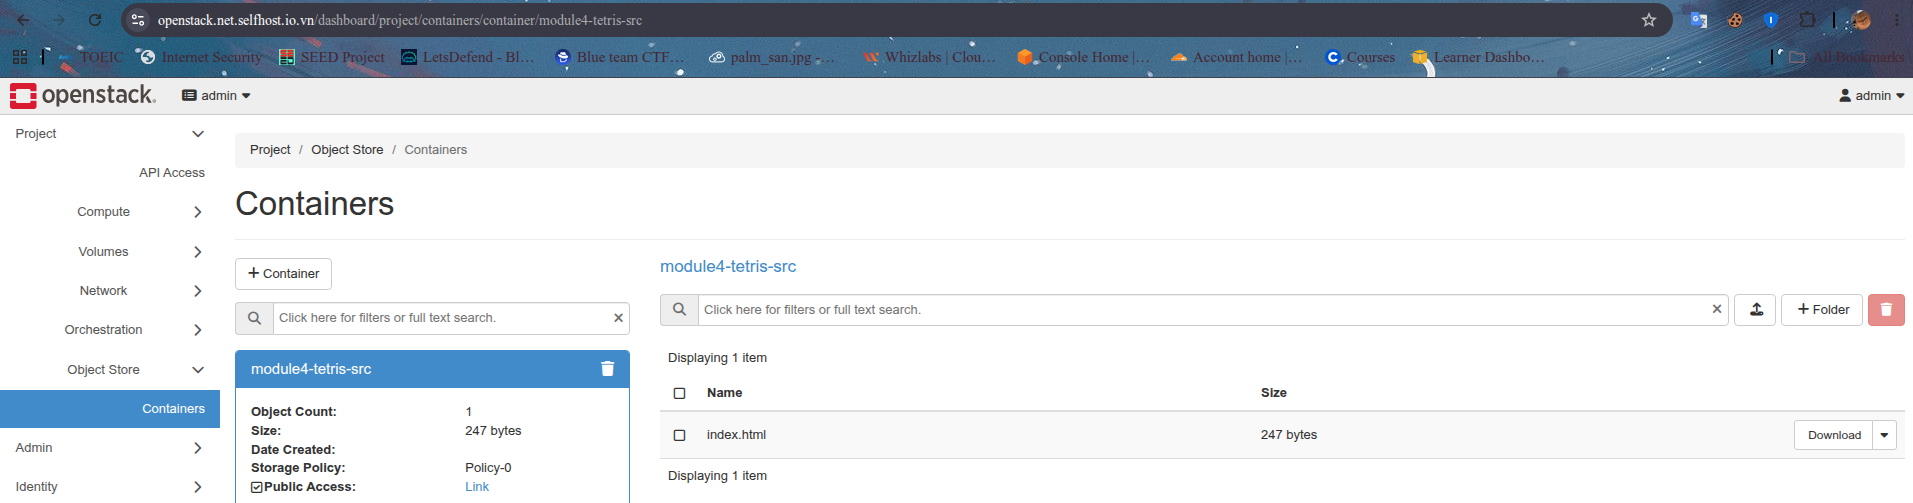
\includegraphics[width=0.88\linewidth]{img/m4-swift-container-object-upload.png}
\caption{Container Swift \texttt{module4-tetris-src} lưu trữ tệp \texttt{index.html} với quyền truy cập public.}
\label{fig:m4_swift_upload}
\end{figure}

\subsection{Tích hợp Cinder Block Volume \& Triển khai Dịch vụ Web}
Sau khi hoàn tất khâu chuẩn bị mã nguồn tĩnh trên Swift, nhóm chúng em tiến hành cấp phát không gian lưu trữ khối bền vững và tích hợp vào máy chủ web:
\begin{enumerate}
    \item \textbf{Khởi tạo \& Gắn Volume:}
    Chúng em tạo một ổ đĩa Cinder dung lượng 1 GiB với định danh \nolinkurl{module4-data-volume} và thực hiện đính kèm (attach) vào máy ảo \texttt{module3-web-sever}. Lớp ảo hóa KVM/QEMU nhận diện thiết bị này dưới định danh \texttt{/dev/vdc} (Hình~\ref{fig:m4_cinder_volume}).
    
    \item \textbf{Định dạng Hệ thống Tệp \& Đồng bộ Mã nguồn (Hình~\ref{fig:m4_vm1_workflow}):}
    Truy cập vào máy ảo thông qua phiên SSH, nhóm chúng em tiến hành định dạng ổ đĩa với hệ thống tệp \texttt{ext4}, tạo thư mục mount \texttt{/mnt/data}, sau đó tải tệp mã nguồn từ endpoint REST của Swift về lưu trữ trực tiếp trên volume:
\begin{lstlisting}[language=bash, basicstyle=\ttfamily\scriptsize]
$ sudo mkfs.ext4 /dev/vdc
$ sudo mkdir -p /mnt/data && sudo mount /dev/vdc /mnt/data
$ cd /mnt/data
$ sudo wget http://192.168.2.10:8080/v1/AUTH_.../module4-tetris-src/index.html
\end{lstlisting}

    \item \textbf{Kích hoạt \& Kiểm thử Dịch vụ Web:}
    Để ứng dụng phục vụ trực tiếp từ ổ đĩa bền vững, chúng em khởi chạy tiến trình BusyBox HTTP daemon với thư mục gốc trỏ vào \texttt{/mnt/data}:
\begin{lstlisting}[language=bash, basicstyle=\ttfamily\scriptsize]
$ sudo busybox httpd -f -p 80 -h /mnt/data &
$ curl http://127.0.0.1
\end{lstlisting}
    Kết quả kiểm tra qua lệnh \texttt{curl} xác nhận máy chủ web đã phản hồi chính xác nội dung HTML được đọc từ phân vùng Cinder.
\end{enumerate}

\begin{figure}[H]
\centering
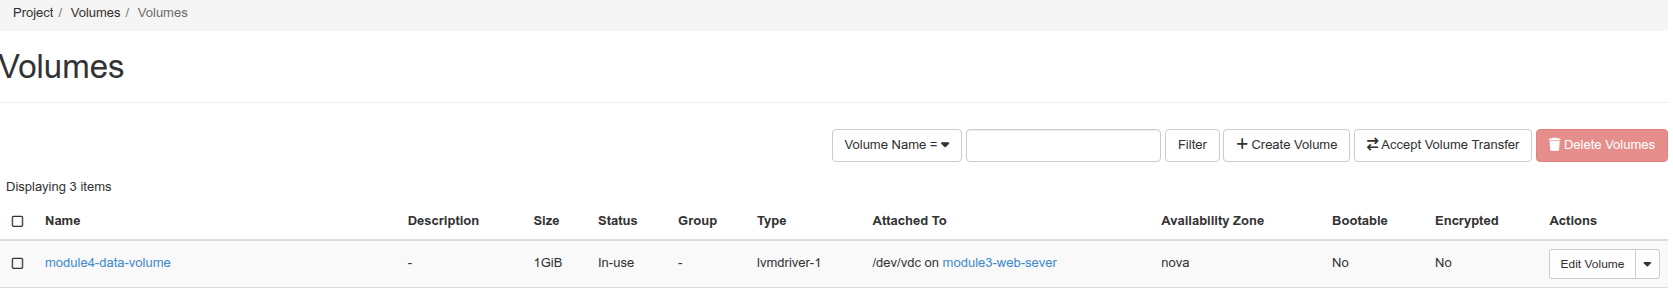
\includegraphics[width=0.88\linewidth]{img/m4-cinder-volume-attached.png}
\caption{Cinder volume \nolinkurl{module4-data-volume} (1 GiB) ở trạng thái In-Use gắn vào \nolinkurl{module3-web-sever}.}
\label{fig:m4_cinder_volume}
\end{figure}

\begin{figure}[H]
\centering
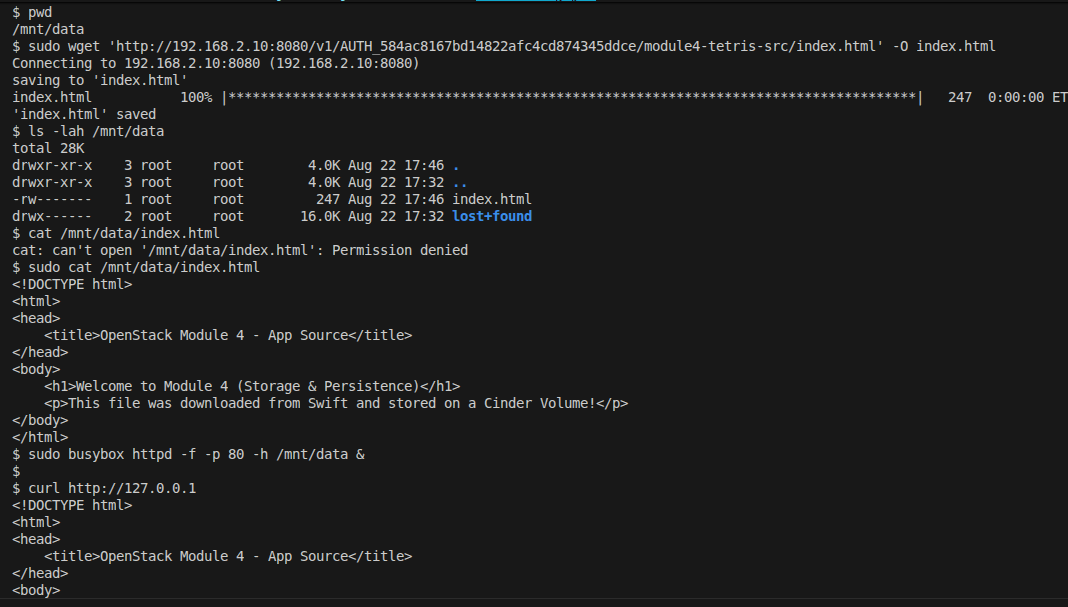
\includegraphics[width=0.88\linewidth]{img/m4-vm1-swift-fetch-cinder-host.png}
\caption{Quy trình terminal: tải mã nguồn từ Swift, mount ổ đĩa Cinder và chạy dịch vụ web.}
\label{fig:m4_vm1_workflow}
\end{figure}

\subsection{Tạo Snapshot \& Xác thực Phục hồi Thảm họa (Disaster Recovery)}
Nhằm chứng minh khả năng bảo toàn dữ liệu và phục hồi hệ thống khi xảy ra sự cố nghiêm trọng trên máy chủ tính toán, nhóm chúng em xây dựng kịch bản cứu hộ dữ liệu độc lập thông qua Snapshot:
\begin{enumerate}
    \item \textbf{Ngắt Kết nối An toàn \& Tạo Snapshot:}
    Để đảm bảo tính toàn vẹn dữ liệu (Data Consistency), chúng em tiến hành unmount hệ thống tệp và detach ổ đĩa khỏi máy ảo ban đầu. Tiếp theo, một bản sao lưu trạng thái thời điểm mang tên \texttt{module4-data-snapshot} (1 GiB) được khởi tạo thành công (Hình~\ref{fig:m4_volume_snapshot}).
    
    \item \textbf{Khôi phục Volume Độc lập từ Snapshot:}
    Từ bản snapshot vừa ghi lại, chúng em tạo ra một ổ đĩa khối mới hoàn toàn độc lập mang tên \nolinkurl{module4-restored-volume}.

    \item \textbf{Khởi tạo Máy ảo Phục hồi Cứu hộ:}
    Chúng em triển khai một máy ảo cứu hộ mới mang tên \nolinkurl{module4-recovery-server} (sử dụng image Fedora Cloud Base) trên phân đoạn mạng \texttt{m2-dmz-net}, sau đó gắn ổ đĩa \nolinkurl{module4-restored-volume} vào máy ảo này.

    \item \textbf{Kiểm tra Tính Toàn vẹn Dữ liệu Cấp độ Byte (Hình~\ref{fig:m4_recovery_verify}):}
    Trên máy ảo phục hồi, nhóm chúng em mount trực tiếp thiết bị \texttt{/dev/vdb} vào thư mục \texttt{/mnt/recovered} mà \textbf{hoàn toàn không cần format lại hệ thống tệp}:
\begin{lstlisting}[language=bash, basicstyle=\ttfamily\scriptsize]
[fedora@module4-recovery-server ~]$ sudo mount /dev/vdb /mnt/recovered
[fedora@module4-recovery-server ~]$ sudo cat /mnt/recovered/index.html
\end{lstlisting}
    Nội dung tệp \texttt{index.html} được đọc ra chính xác tuyệt đối từng byte. Thực nghiệm này chứng minh cơ chế Snapshot của Cinder bảo vệ dữ liệu nguyên vẹn 100\%, giúp hệ thống sẵn sàng phục hồi ngay cả khi node tính toán ban đầu bị phá hủy hoàn toàn.
\end{enumerate}

\begin{figure}[H]
\centering
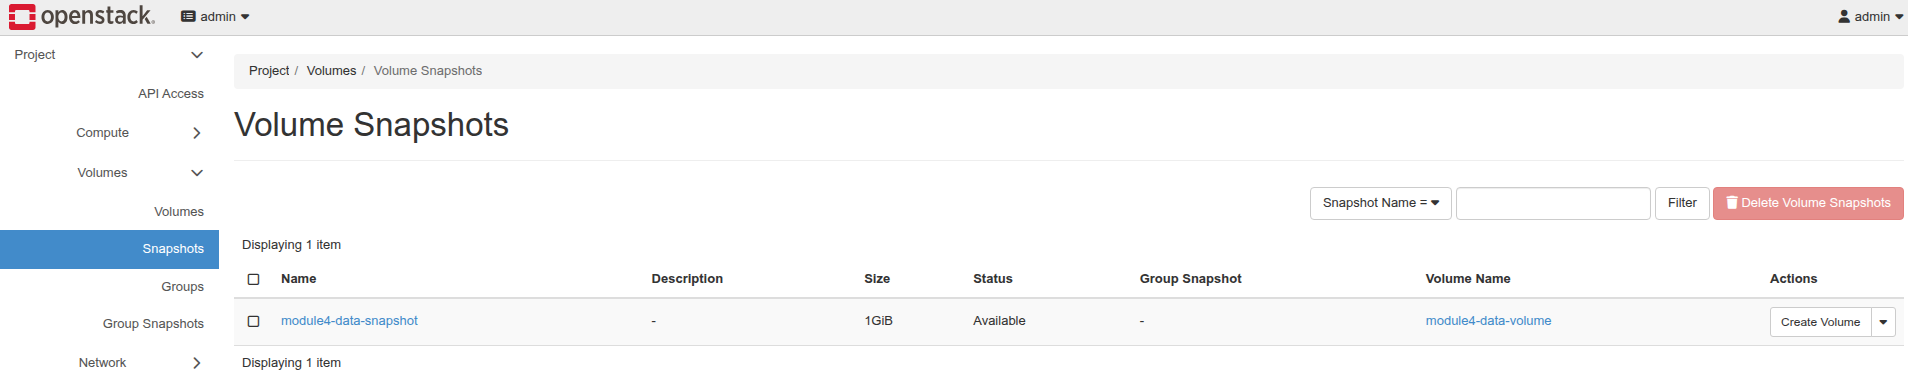
\includegraphics[width=0.88\linewidth]{img/m4-cinder-volume-snapshot.png}
\caption{Bản snapshot \texttt{module4-data-snapshot} ghi nhận trạng thái ổ đĩa tại thời điểm sao lưu.}
\label{fig:m4_volume_snapshot}
\end{figure}

\begin{figure}[H]
\centering
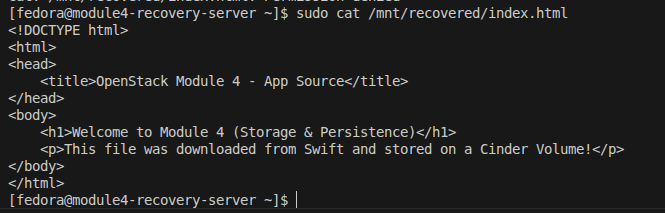
\includegraphics[width=0.88\linewidth]{img/m4-recovery-server-data-verification.png}
\caption{Kiểm tra tính toàn vẹn trên máy ảo phục hồi xác nhận dữ liệu được bảo toàn nguyên vẹn.}
\label{fig:m4_recovery_verify}
\end{figure}


